\documentclass{article}

\usepackage{fullpage}
\usepackage{graphicx}

\title{A review of steer torque measurements in bicycles and motorcycles}
\author{Jason K. Moore and Mont Hubbard}
\date{\today}

\begin{document}

\maketitle

Applying forces to the handlebars of motorcycles and bicycles which cause
rotation of the front frame about the steer axis provide the most authority of
any other input for control of the vehicles. It is also clear that haptic
feedback is near essential for a human to balance a bicycle, i.e. with only
position control of the handlebars the rider cannot maintain balance. Thus is
it critical to understand the steer torque to understand botht he open loop and
closed loop dynamics of the bicycle/motorcycle-rider system.

The first portion of the paper will be devoted to a detailed review of steer
torque measurements. The earliest measurements of steer torque were done on a
motorcycle by \cite{Wilson-Jones1951}, followed by \cite{Kondo1955}. There have
since various measurements of steer torque, mostly on motorcycles and a few on
bicycles.

The applied steer torque need to control a motorcycle is much greater in
magnitude for that of a bicycle. 0-50 Nm for motorcycles and 0-10 Nm for
similar manuevers on bicycles. Furthermore the rider can easily apply moments
other than steer torque to the handlebars of up to 200 Nm. The sensor design
must designed such that these other moments do not corrupt the much lower
magintued steer torque measurements which are desired.

There are three main designs for measuring steer torque: forces at the
hand-handlebar interface, torque transducers on the steer axis, beam
transducers.

We show that careful attention must be made to any steer torque sensors which
measure the strains at points between the hands and the contact point.
Depending on the location along the steer axis that the measurement is made,
the interial effects of front frame and handlebars between the sensor and teh
rider's hands must be accounted for. For bicycles this is very important
because the torques due to the inerital effects can be a high percentage of the
actual applied torque. No previous steer torqe measurements seem to take this
into account.

\begin{figure}
  \centering
  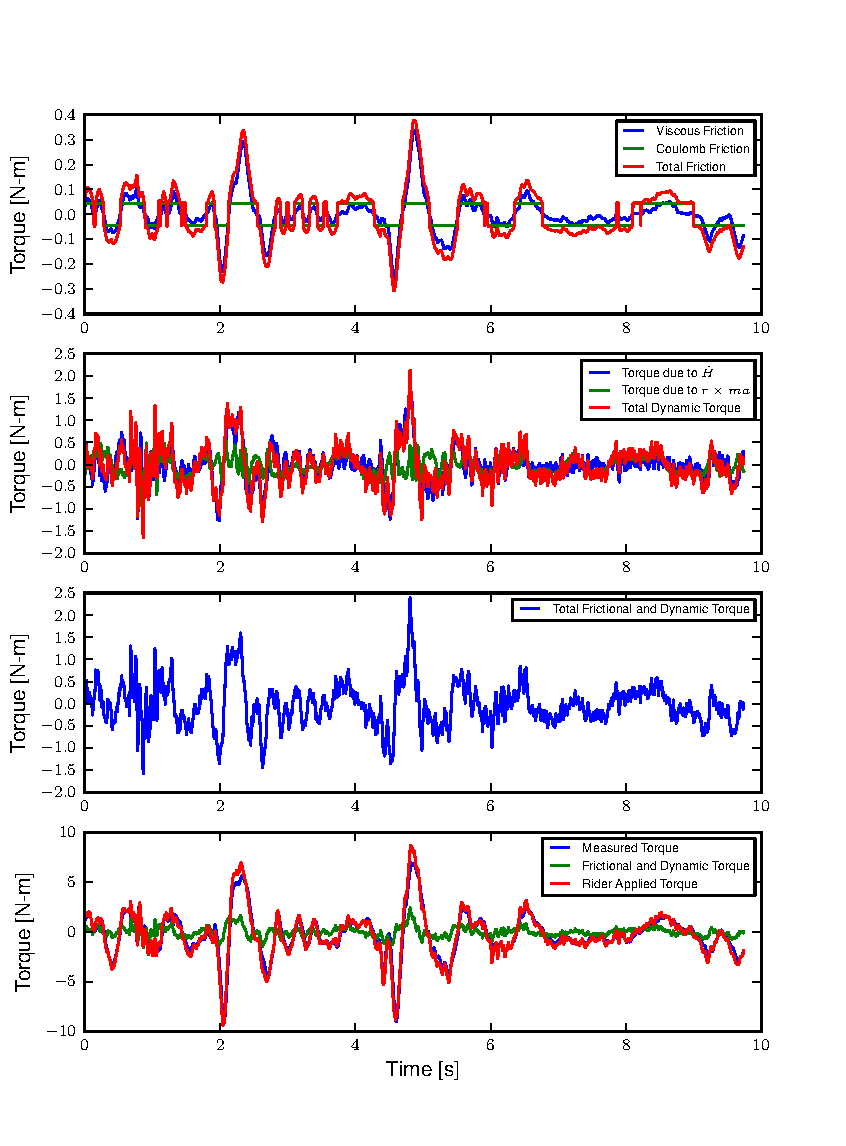
\includegraphics{steer-torque-components.pdf}
  \caption{This is a plot of the steer torque components for run \#700. The top
  plot shows the additive viscous and Coulomb friction. The total bearing
  friction during the run is less 0.3 Nm. The second plot shows the torque the
  rider must apply to overcome the handlebar inertia. The dominant term is the
  $I_{G_{33}} w_{b3}$ and during the peak accelerations the additive torque is
  up to 1.5 Nm for this run. The third plot shows the total additive torque
  which is up to 2 Nm. And finally the last plot shows the difference in the
  measured torque and the rider applied torque. There are large differences,
  especially at the peaks.}
\end{figure}

Finally, we will show the steer torque measurement sensor designed for an
instrumented bicycle which attempts to take into account many of the flaws of
previous measurements and we show results for very accurate torque measurements
in various bicycle manuevers.

This paper is based on work supported by the National Science Foundation under
Grant No 0928339.

\bibliographystyle{plain}
\bibliography{bicycle}

\end{document}
